% =====================================================================
%  ch01_overview.tex -- 第 1 章 工程总览
% =====================================================================
\section{工程总览}

\subsection{本报告的范围与方法}

本报告针对 \file{project_2025_11_07} 这一 Gowin（高云）FPGA 工程，逐文件、逐语句块地
解析其 RTL 设计。分析对象为工程文件中列出的全部 11 个 Verilog 源文件、2 个 IP 生成文件、
1 个物理约束文件，以及工程目录中附带的 2 个 IP 例化模板：

\begin{center}
\small
\begin{tabular}{llc}
\toprule
类别 & 文件 & 是否进入网表\\
\midrule
顶层 & \file{src/adda.v} & 是（Top）\\
算法 & \file{src/rtl.v}、\file{src/eso.v} & 是\\
外设 & \file{src/uart_rx.v}、\file{src/uart_tx.v} & 是\\
显示 & \file{src/seg.v}、\file{src/bcd.v} & 是\\
基础 & \file{src/key.v}、\file{src/divider.v} & 是\\
IP & \file{src/gowin_pll/gowin_pll.v} & 否（未例化）\\
IP & \file{src/fifo_top/fifo_top.v} & 否（未例化）\\
约束 & \file{src/project_2025_11_07.cst} & 引脚/电平\\
模板 & \file{src/gowin_pll/gowin_pll_tmp.v}、\file{src/fifo_top/fifo_top_tmp.v} & 否（仅供查阅）\\
\bottomrule
\end{tabular}
\end{center}

“进入网表”一列并非主观判断，而是由三处证据共同确认：综合资源报告
\file{syn_rsc.xml} 中只出现 7 个子模块；PnR 报告 \file{rpt.txt} 中 PLL 占用为
\sig{0/6}、BSRAM 占用为 0\%；以及 \file{adda.v} 中 \sig{Gowin_PLL}、\sig{fifo_top}
的例化代码被注释符包裹（完整路径见第 1.2 节的目录说明）。

解析方法遵循“自顶向下、逐块下钻”的原则，每一章的结构固定为：
\begin{enumerate}[leftmargin=2em,itemsep=2pt]
  \item \textbf{文件信息}：路径、模块名、实例名、行数、时序模板；
  \item \textbf{模块接口（第 1 层）}：端口表、参数表；
  \item \textbf{内部结构（第 2 层）}：寄存器/连线清单与语句块索引；
  \item \textbf{语句块解析（第 3 层）}：每块给出现行代码、逐信号解释、数值与时序推演；
  \item \textbf{要点与风险}：设计意图、隐含假设、潜在缺陷。
\end{enumerate}

\subsection{工程来源、工具链与“用 TD 打开”的说明}

\subsubsection{原始工程}

工程由 Gowin EDA（云源软件）V1.9.9 64-bit 生成，工程主文件为
\file{project_2025_11_07.gprj}，其 \sig{<Device>} 节点写明了器件：

\begin{lstlisting}[style=cfgcode,numbers=none]
<Device name="GW5A-25A" pn="GW5A-LV25UG324C2/I1">gw5a25a-008</Device>
\end{lstlisting}

综合工程文件还给出了封装与速度等级：
\begin{lstlisting}[style=cfgcode,numbers=none]
<Device id="GW5A-25A" package="UBGA324" speed="2" partNumber="GW5A-LV25UG324C2/I1"/>
\end{lstlisting}

\subsubsection{关于用安路 TD 打开该工程}

这里需要明确一个前提：\textbf{安路 TangDynasty（TD）无法直接打开高云的 \texttt{.gprj} 工程}。
两者是不同厂商的私有工程格式（高云 \sig{.gprj} / 安路 \sig{.al}），器件库、原语、IP 格式、
约束语言（高云 \sig{.cst} 与安路 \sig{.adc}/\sig{.fdc}）均不兼容。经检查，本机安装的是
\textbf{TD 6.0.3 PHX SP2}，其器件数据库 \file{D:\textbackslash FPGA\textbackslash arch\textbackslash device_resource\textbackslash device_resource.csv}
只包含 \sig{ph1}（13 个）与 \sig{ph2}（2 个）两个 Phoenix 系列，不含 GW5A 或任何高云器件。

因此本次采用“\textbf{同名工程容器}”的方案：用 TD 的 Tcl 接口
（\file{td_commands_prompt.exe -nogui}）新建了一个与源码同名的 TD 工程
\file{FPGA_TD/project_2025_11_07_TD.al}，器件选用 TD 6.0.3 中规模最小、封装同为 324 球的
\sig{PH1A60GEG324-3}，再把 11 个 Verilog 源文件以\textbf{引用方式}（不复制）加入工程。
这样 TD 的层次树、源码浏览器、交叉引用功能都能用于阅读和注释本工程的代码，而
\textbf{原始高云工程完全未被改动}。

\begin{figure}[htbp]
\centering
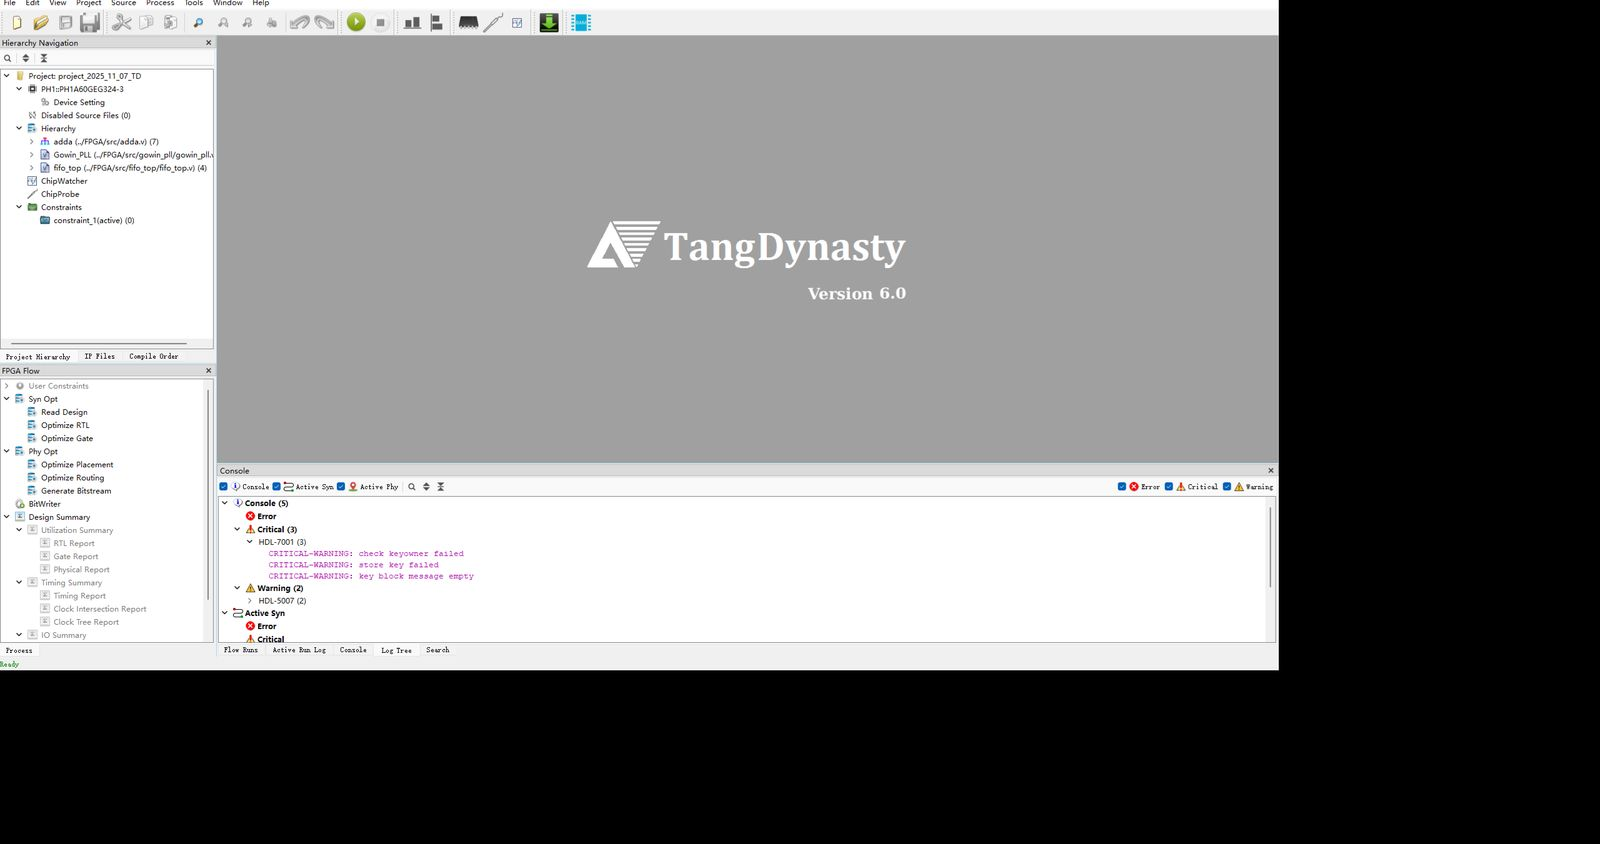
\includegraphics[width=0.92\linewidth]{figs/TD_open_project.jpg}
\caption{TD 6.0.3 打开同名工程容器后的界面：左侧 Hierarchy Navigation 已经识别出
\sig{adda (7)}、\sig{Gowin_PLL (1)}、\sig{fifo_top (4)} 三个层次根，说明全部源文件均被正确解析。}
\label{fig:td-open}
\end{figure}

\begin{tipbox}
\textbf{为什么层次树里 \sig{adda} 只有 7 个子节点？}
因为顶层只例化了 7 个模块（key、seg、rtl、eso、uart\_rx、uart\_tx、divider）。
\sig{Gowin_PLL} 与 \sig{fifo_top} 虽然被 TD 解析并单独列在层次树中，但它们是“未被例化的
孤立模块”，不会出现在 \sig{adda} 之下，也不会进入综合网表——这与高云综合报告的结论一致。
\end{tipbox}

\begin{warnbox}
\textbf{注意}：TD 容器工程只用于“阅读/结构化浏览”代码，\textbf{不要}用它做综合或生成码流。
一方面它选用的是安路 PH1 器件，与板上的 GW5A-25A 引脚、电气属性完全不同；另一方面
\sig{gowin_pll.v} 里的 \sig{PLLA} 原语和 \sig{fifo_top.v} 里加密的 FIFO 都不属于安路器件库。
若需要重新编译，应回到 Gowin EDA 打开原始 \sig{.gprj}。
\end{warnbox}

\subsection{器件与资源}

\begin{table}[htbp]
\centering
\small
\caption{GW5A-LV25UG324C2/I1 的容量与本工程占用}
\begin{tabular}{lrr}
\toprule
资源 & 器件容量 & 本工程占用\\
\midrule
LUT / ALU / ROM16（逻辑） & 23\,040 & 575（2\%）\\
寄存器（FF） & 23\,685 & 375（2\%）\\
CLS（逻辑簇） & 11\,520 & 405（4\%）\\
DSP（MULTALU27X18） & 28 & 7（25\%）\\
PLL & 6 & 0（0\%）\\
BSRAM & 若干 & 0（0\%）\\
I/O 端口 & — & 44（其中 42 个实际布出 Buffer）\\
\bottomrule
\end{tabular}
\end{table}

该器件属于 Arora V（GW5A）系列 22nm 工艺的入门型号，324 球 UBGA 封装，速度等级 2，
工业级/商业级双标注（C2/I1）。工程中真正消耗资源的核心是 \sig{eso.v} 的 9 个乘法器
（映射为 7 个 MULTALU27X18）与 \sig{rtl.v} 的两个除法器，其余模块都是控制/IO 逻辑。

\subsection{模块层次与文件对应关系}

\begin{figure}[htbp]
\centering
\begin{minipage}{0.9\linewidth}
\begin{verbatim}
adda  (src/adda.v)                              <- 顶层 / Top Module
 |-- key_inst      : key      (src/key.v)        按键消抖 20ms
 |-- seg_inst      : seg      (src/seg.v)        数码管动态扫描
 |    `-- bcd_8421 : bcd      (src/bcd.v)        二进制 -> 3 位 BCD
 |-- adc_inst      : rtl      (src/rtl.v)        中值滤波 + 电压换算
 |-- eso_inst      : eso      (src/eso.v)        扩展状态观测器 (ADRC)
 |-- uart_rx_inst  : uart_rx  (src/uart_rx.v)    串口接收 (8N1)
 |-- uart_tx_inst  : uart_tx  (src/uart_tx.v)    串口发送 (16bit)
 `-- divider_inst  : divider  (src/divider.v)    1kHz 分频

未例化(只在工程文件列表里): Gowin_PLL (gowin_pll.v) / fifo_top (fifo_top.v)
\end{verbatim}
\end{minipage}
\caption{模块层次树。带 \texttt{--} 前缀的是实例名，括号内为源文件。}
\label{fig:hier}
\end{figure}

\begin{table}[htbp]
\centering
\small
\caption{例化关系与实例名一览}
\begin{tabular}{llll}
\toprule
父模块 & 子模块 & 实例名 & 作用\\
\midrule
adda & key & key\_inst & 按键消抖 \\
adda & seg & seg\_inst & 数码管扫描显示 \\
seg & bcd & bcd\_8421 & 二进制转 BCD \\
adda & rtl & adc\_inst & 中值/电压换算 \\
adda & eso & eso\_inst & 扩展状态观测器 \\
adda & uart\_rx & uart\_rx\_inst & 串口接收 \\
adda & uart\_tx & uart\_tx\_inst & 串口发送 \\
adda & divider & divider\_inst & 1kHz 分频 \\
\bottomrule
\end{tabular}
\end{table}

\subsection{数据流与控制流}

系统是一套“AD 采样 $\rightarrow$ 数字化处理 $\rightarrow$ DA 回放 + 显示 + 串口上报 + 上位机在线调参”
的闭环演示平台：

\begin{figure}[htbp]
\centering
\begin{minipage}{0.95\linewidth}
\begin{verbatim}
  [外部 ADC] --ad_date[9:0]--> rtl (中值/电压) --sign--> seg(+bcd) --> 数码管
  [外部 ADC] --ad_date[9:0]--> date_y(=ad_date-512) --> eso(1kHz)
                --date_u--> (~u + 512) --> DAC ad_out[9:0]
  [上位机 rx] --Axxx/Bxxx--> uart_rx --> 16bit 组帧 --> c_date/k_date --> eso
  [按键 key_in] --> key --> key_out --> 选择 ad_out 的数据来源
  [ad_date] --> uart_tx --> tx (115200, 8N1, 每帧 182us)
  [sys_clk 50MHz] --> divider --> ad_clk1/da_clk1 (1kHz) --> eso 采样时钟
\end{verbatim}
\end{minipage}
\caption{数据流与控制关系（省略复位线与时钟树细节）。}
\label{fig:dataflow}
\end{figure}

\begin{table}[htbp]
\centering
\small
\caption{关键信号与跨模块连接}
\begin{tabular}{lp{3.2cm}p{6.4cm}}
\toprule
信号 & 位宽/类型 & 说明\\
\midrule
\sig{ad_date[9:0]} & 10bit 无符号 & 外部 ADC 并行码值（偏移二进制，中点 512）\\
\sig{date_y} & 10bit 有符号 & \sig{ad_date-512}，把中点移到零，送 ESO 的误差输入\\
\sig{date_u} & 10bit 有符号 & ESO 输出的控制量，同时回送 ESO 的 \sig{u_out} 形成反馈\\
\sig{ad_out[9:0]} & 10bit 无符号 & 送 DAC 的偏移二进制码，由按键选择“直通”或“控制量”\\
\sig{c_date/k_date} & 12bit & 串口下发的两个 ESO 参数（A 帧、B 帧的低 12 位）\\
\sig{po_data/po_flag} & 8bit/1bit & 串口接收字节与单周期有效脉冲\\
\sig{sign} & 1bit & 当前码值低于中值，数码管据此显示负号\\
\bottomrule
\end{tabular}
\end{table}

\subsection{时钟与复位策略}

\begin{table}[htbp]
\centering
\small
\caption{时钟域一览}
\begin{tabular}{llll}
\toprule
时钟 & 频率 & 来源 & 使用者\\
\midrule
\sig{sys_clk} & 50MHz & 板载有源晶振，引脚 T9 & adda、key、seg、uart\_rx、uart\_tx、divider\\
\sig{ad_clk1} & 1kHz & divider 由 \sig{sys_clk} 分频 & AD 芯片转换时钟、eso 运算时钟\\
\sig{da_clk1} & 1kHz & divider（与 \sig{ad_clk1} 同相） & DA 芯片转换时钟\\
\bottomrule
\end{tabular}
\end{table}

全设计只有一个异步复位 \sig{sys_rst_n}（低有效，引脚 A15），所有时序块都采用
“\sig{posedge clk or negedge rst_n}”的异步复位、同步释放风格（除 \sig{eso} 用
\sig{ad_clk} 作为时钟外）。由于 \sig{ad_clk1} 由 \sig{sys_clk} 分频而来，它与
\sig{sys_clk} 是同源的，1kHz 下不存在实际跨时钟域问题，但用“分频时钟”而非
“时钟使能”驱动的写法在更高频率下需要谨慎（见第 14 章）。

\subsection{参数与定点数约定汇总}

\begin{table}[htbp]
\centering
\small
\caption{全工程参数/常数}
\begin{tabular}{llll}
\toprule
位置 & 名称 & 取值 & 含义\\
\midrule
adda & \sig{CNT_DATA_MAX} & 1024 & 中值样本数（转发给 rtl 的约定值）\\
adda & \sig{CNT_MAX} & 1\,299\,999 & 26ms 定时器（仅驱动死信号 \sig{pi_flag}）\\
divider & \sig{cnt_max} & 24\,999 & $50\text{MHz}/(2\times25000)=1\text{kHz}$\\
key & \sig{CNT_MAX} & 999\,999 & 20ms 消抖时间\\
seg & \sig{CNT_MAX} & 23\,999 & 0.48ms 位扫描间隔\\
bcd & — & 22 拍 & 一次二进制转 BCD 的时钟数\\
uart\_rx/tx & \sig{UART_BPS} & 115\,200 & 波特率\\
uart\_rx/tx & \sig{CLK_FREQ} & 50\,000\,000 & 系统时钟，用于算分频\\
eso & \sig{B01/B02/B03} & 90 / 2700 / 27000 & 观测器增益（配合 $h=2^{-10}$）\\
eso & \sig{b0} & 5000 & 控制增益（配合 $>>13$）\\
eso & \sig{c} / \sig{k} & 150 / 20 & 状态误差反馈参数（可串口在线修改）\\
\bottomrule
\end{tabular}
\end{table}

工程中所有运算均为“整数 + 移位”的定点数，没有浮点。约定如下：
\begin{itemize}[leftmargin=2em,itemsep=1pt]
  \item \sig{rtl} 中电压量的标度为 $100\times$（即 1 LSB = 0.01V），满量程 $\pm2.0$V；
  \item \sig{eso} 中采样步长 $h=1/1024$ 由 \sig{>>>10} 实现，系数 \sig{B0x} 直接乘后右移；
  \item \sig{eso} 输出经 \sig{>>>15} 压缩后取低 10 位，映射到 DAC 的 0$\sim$1023 量程。
\end{itemize}

\subsection{代码风格与工程约定}

\begin{itemize}[leftmargin=2em,itemsep=2pt]
  \item \textbf{时序模板}：几乎所有状态块都是“复位分支 + else if 条件 + else 保持”结构，
        属于安全的默认保持型写法，综合后不会产生锁存器；
  \item \textbf{位宽}：大量使用 \sig{<= 1'b0} 给多位寄存器赋初值（例如
        \sig{data_reg<=1'b0}），Verilog 会自动零扩展，功能正确但不是严谨写法；
  \item \textbf{命名}：沿用“中文注释 + 拼音变量”（\sig{date}、\sig{pingj}、\sig{seg_date}），
        阅读时需要对照注释理解；
  \item \textbf{重复常量}：\sig{50_000_000} 在 uart 例化处出现两次，\sig{115200} 同样，
        若更换时钟需同步修改 PLL 参数、divider 参数与 uart 参数三处。
\end{itemize}
